\documentclass[aspectratio=169,11pt]{beamer}
\usetheme{Madrid}
\usecolortheme{default}
\usepackage{amsmath,amssymb,booktabs}
\usepackage{graphicx}
\usepackage{tikz}
\usepackage{listings}
\definecolor{navy}{RGB}{16,42,68}
\definecolor{teal}{RGB}{0,111,116}
\definecolor{pale}{RGB}{239,246,246}
\setbeamercolor{structure}{fg=navy}
\setbeamercolor{frametitle}{fg=white,bg=navy}
\setbeamercolor{block title}{fg=white,bg=teal}
\setbeamercolor{block body}{fg=navy,bg=pale}
\setbeamertemplate{navigation symbols}{}
\setbeamertemplate{footline}{}
\setbeamertemplate{headline}{}
\setbeamertemplate{itemize item}{\color{teal}$\blacktriangleright$}
\lstset{basicstyle=\ttfamily\scriptsize,breaklines=true,frame=single,
  rulecolor=\color{teal},keywordstyle=\color{navy}\bfseries}
\title{The Race between Man and Machine}
\subtitle{Tasks, wages, and what a formal proof can establish}
\author{John Barraza}
\date{Repository 6 \quad | \quad September 2026}
\begin{document}

\begin{frame}
\titlepage
\centering\small\url{https://github.com/johnbarraza/ai-06-restrepo}
\end{frame}

\begin{frame}{Road map for 20 minutes}
\begin{enumerate}
\item The aggregate task economy and equilibrium threshold
\item Automation versus new tasks: opposite reallocations
\item The wage condition, its analytical and numerical check
\item Lean translation: checked theorem, proof step, and limits
\item Hand verification and verdict
\end{enumerate}
\end{frame}

\begin{frame}{Question and unit of analysis}
\begin{block}{Question}
Can automation raise output yet lower the wage? Can new tasks reverse the fall in labor's share?
\end{block}
\vspace{.5em}
Unlike the earlier weekly papers, the unit here is the \alert{aggregate economy}: a continuum of production tasks and competitive factor markets.
\end{frame}

\begin{frame}{The task space}
\centering
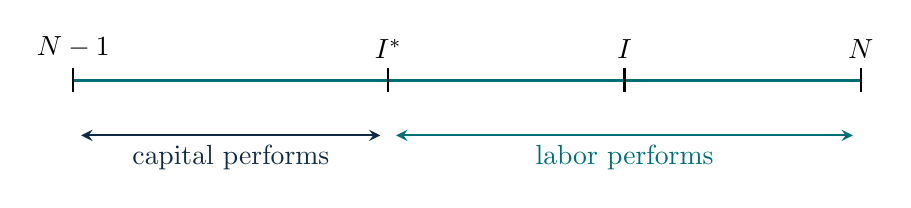
\begin{tikzpicture}[>=stealth,scale=1]
\draw[very thick,teal] (0,0)--(10,0);
\draw[thick] (0,-.15)--(0,.15) node[above] {$N-1$};
\draw[thick] (4,-.15)--(4,.15) node[above] {$I^*$};
\draw[thick] (7,-.15)--(7,.15) node[above] {$I$};
\draw[thick] (10,-.15)--(10,.15) node[above] {$N$};
\draw[<->,navy,thick] (.1,-.7)--(3.9,-.7) node[midway,below] {capital performs};
\draw[<->,teal,thick] (4.1,-.7)--(9.9,-.7) node[midway,below] {labor performs};
\end{tikzpicture}
\vspace{1em}
\begin{block}{Two frontiers}
$I$ is technological feasibility; $I^*$ is actual capital use. They need not coincide.
\end{block}
\end{frame}

\begin{frame}{The agents' problems}
\begin{columns}[T]
\column{.49\textwidth}
\textbf{Competitive task producer}
\vspace{.4em}
For $i\le I$, compare factor costs
\vspace{.3em}
\[\min\left\{R,\frac{W}{\gamma(i)}\right\}.\]
For $i>I$, only labor is feasible. Intermediate inputs also enter full unit cost.
\column{.49\textwidth}
\textbf{Representative household}
\vspace{.4em}
Choose $(C,L)$ with $C=WL+RK$ to maximize the paper's $u(C,L)$. At an interior choice:
\[\nu'(L)=\frac{W}{C}.\]
\end{columns}
\end{frame}

\begin{frame}{Comparative advantage implies a threshold}
\[\frac{W}{R}=\gamma(\widetilde I),\qquad I^*=\min\{I,\widetilde I\}.\]
\begin{itemize}
\item $\gamma(i)$ strictly increases: labor has an advantage in more complex tasks.
\item Below $I^*$: capital is cheaper; above $I^*$: labor is used.
\item If $I<\widetilde I$, technology constrains automation.
\item If $\widetilde I<I$, technology is slack; more feasible automation changes nothing locally.
\end{itemize}
\end{frame}

\begin{frame}{Conditions behind the static results}
\begin{enumerate}
\item $\gamma(i)$ strictly increasing (Assumption 1).
\item $\eta\to0$ or $\zeta=1$ (Assumption 2): homothetic factor demand.
\item $K<\bar K$ (Assumption 3): new tasks are used.
\end{enumerate}
\vspace{.6em}
$\sigma>0$, $\widehat\sigma>0$, $\varepsilon_L>0$, and the household's convexity and regularity conditions also matter. Proposition 1 supplies a unique static equilibrium under these conditions.
\end{frame}

\begin{frame}{Automation and reinstatement}
\begin{columns}[T]
\column{.49\textwidth}
\begin{block}{Automation: $I\uparrow$}
Capital takes over some existing labor tasks. In the constrained regime, $W/R$, labor share, and employment fall.
\end{block}
\column{.49\textwidth}
\begin{block}{New tasks: $N\uparrow$}
New complex tasks require labor and replace low-index tasks. $W/R$, labor share, employment, and the wage rise.
\end{block}
\end{columns}
\vspace{.7em}
These are Proposition 2--3 static comparative statics, not unconditional predictions for a dynamic economy.
\end{frame}

\begin{frame}{The wage trap: two forces}
\[\underbrace{\frac{d\ln W}{dI}}_{\text{wage response}}
=\underbrace{P_I}_{\text{productivity gain}}
-\underbrace{\frac{(1-s_L)\Lambda_I}{\widehat\sigma+\varepsilon_L}}_{\text{displacement}}.\]
\begin{block}{Exact local condition, $I^*=I<\widetilde I$}
The wage rises iff
\[P_I>\frac{(1-s_L)\Lambda_I}{\widehat\sigma+\varepsilon_L}.\]
Equality gives no local change; a reversed inequality gives a fall.
\end{block}
\end{frame}

\begin{frame}{A different sign is fixed}
\[\frac{d\ln(W/R)}{dI}=-\frac{\Lambda_I}{\widehat\sigma+\varepsilon_L}<0.\]
The labor share and employment move with $\omega=W/(RK)$ and therefore fall in the constrained case.
\vspace{.8em}
\begin{alertblock}{Interpretation}
A falling labor share does not prove that the \emph{level} of the real wage falls. Productivity and displacement compete in the wage equation.
\end{alertblock}
\end{frame}

\begin{frame}{Analytical and computational check}
\begin{center}
\begin{tabular}{lccc}
\toprule
Illustrative case & $P_I$ & displacement & $d\ln W/dI$ \\
\midrule
Large productivity gain & .400 & .133 & +.267 \\
Small productivity gain & .050 & .133 & $-.083$ \\
Equality & .133 & .133 & $0$ \\
\bottomrule
\end{tabular}
\end{center}
\vspace{.4em}
Same $s_L=.6$, $\Lambda_I=.5$, $\widehat\sigma=1$, $\varepsilon_L=.5$ in every row. Reproduce with \texttt{python analysis/wage\_condition.py}. These inputs illustrate the sign identity; they are not solved equilibria.
\end{frame}

\begin{frame}{Where I did not trust the AI}
\begin{alertblock}{Claim to test}
``Automation necessarily reduces wages and labor's share.''
\end{alertblock}
\begin{itemize}
\item Labor share falls only when the automation frontier binds; at a slack frontier, a small increase in $I$ has no effect.
\item The wage can rise when the productivity gain dominates displacement.
\item At $I^*=I=\widetilde I$, use one-sided derivatives.
\end{itemize}
\end{frame}

\begin{frame}{Hand check: the decisive inequality}
\IfFileExists{hand/derivation.jpg}{\centering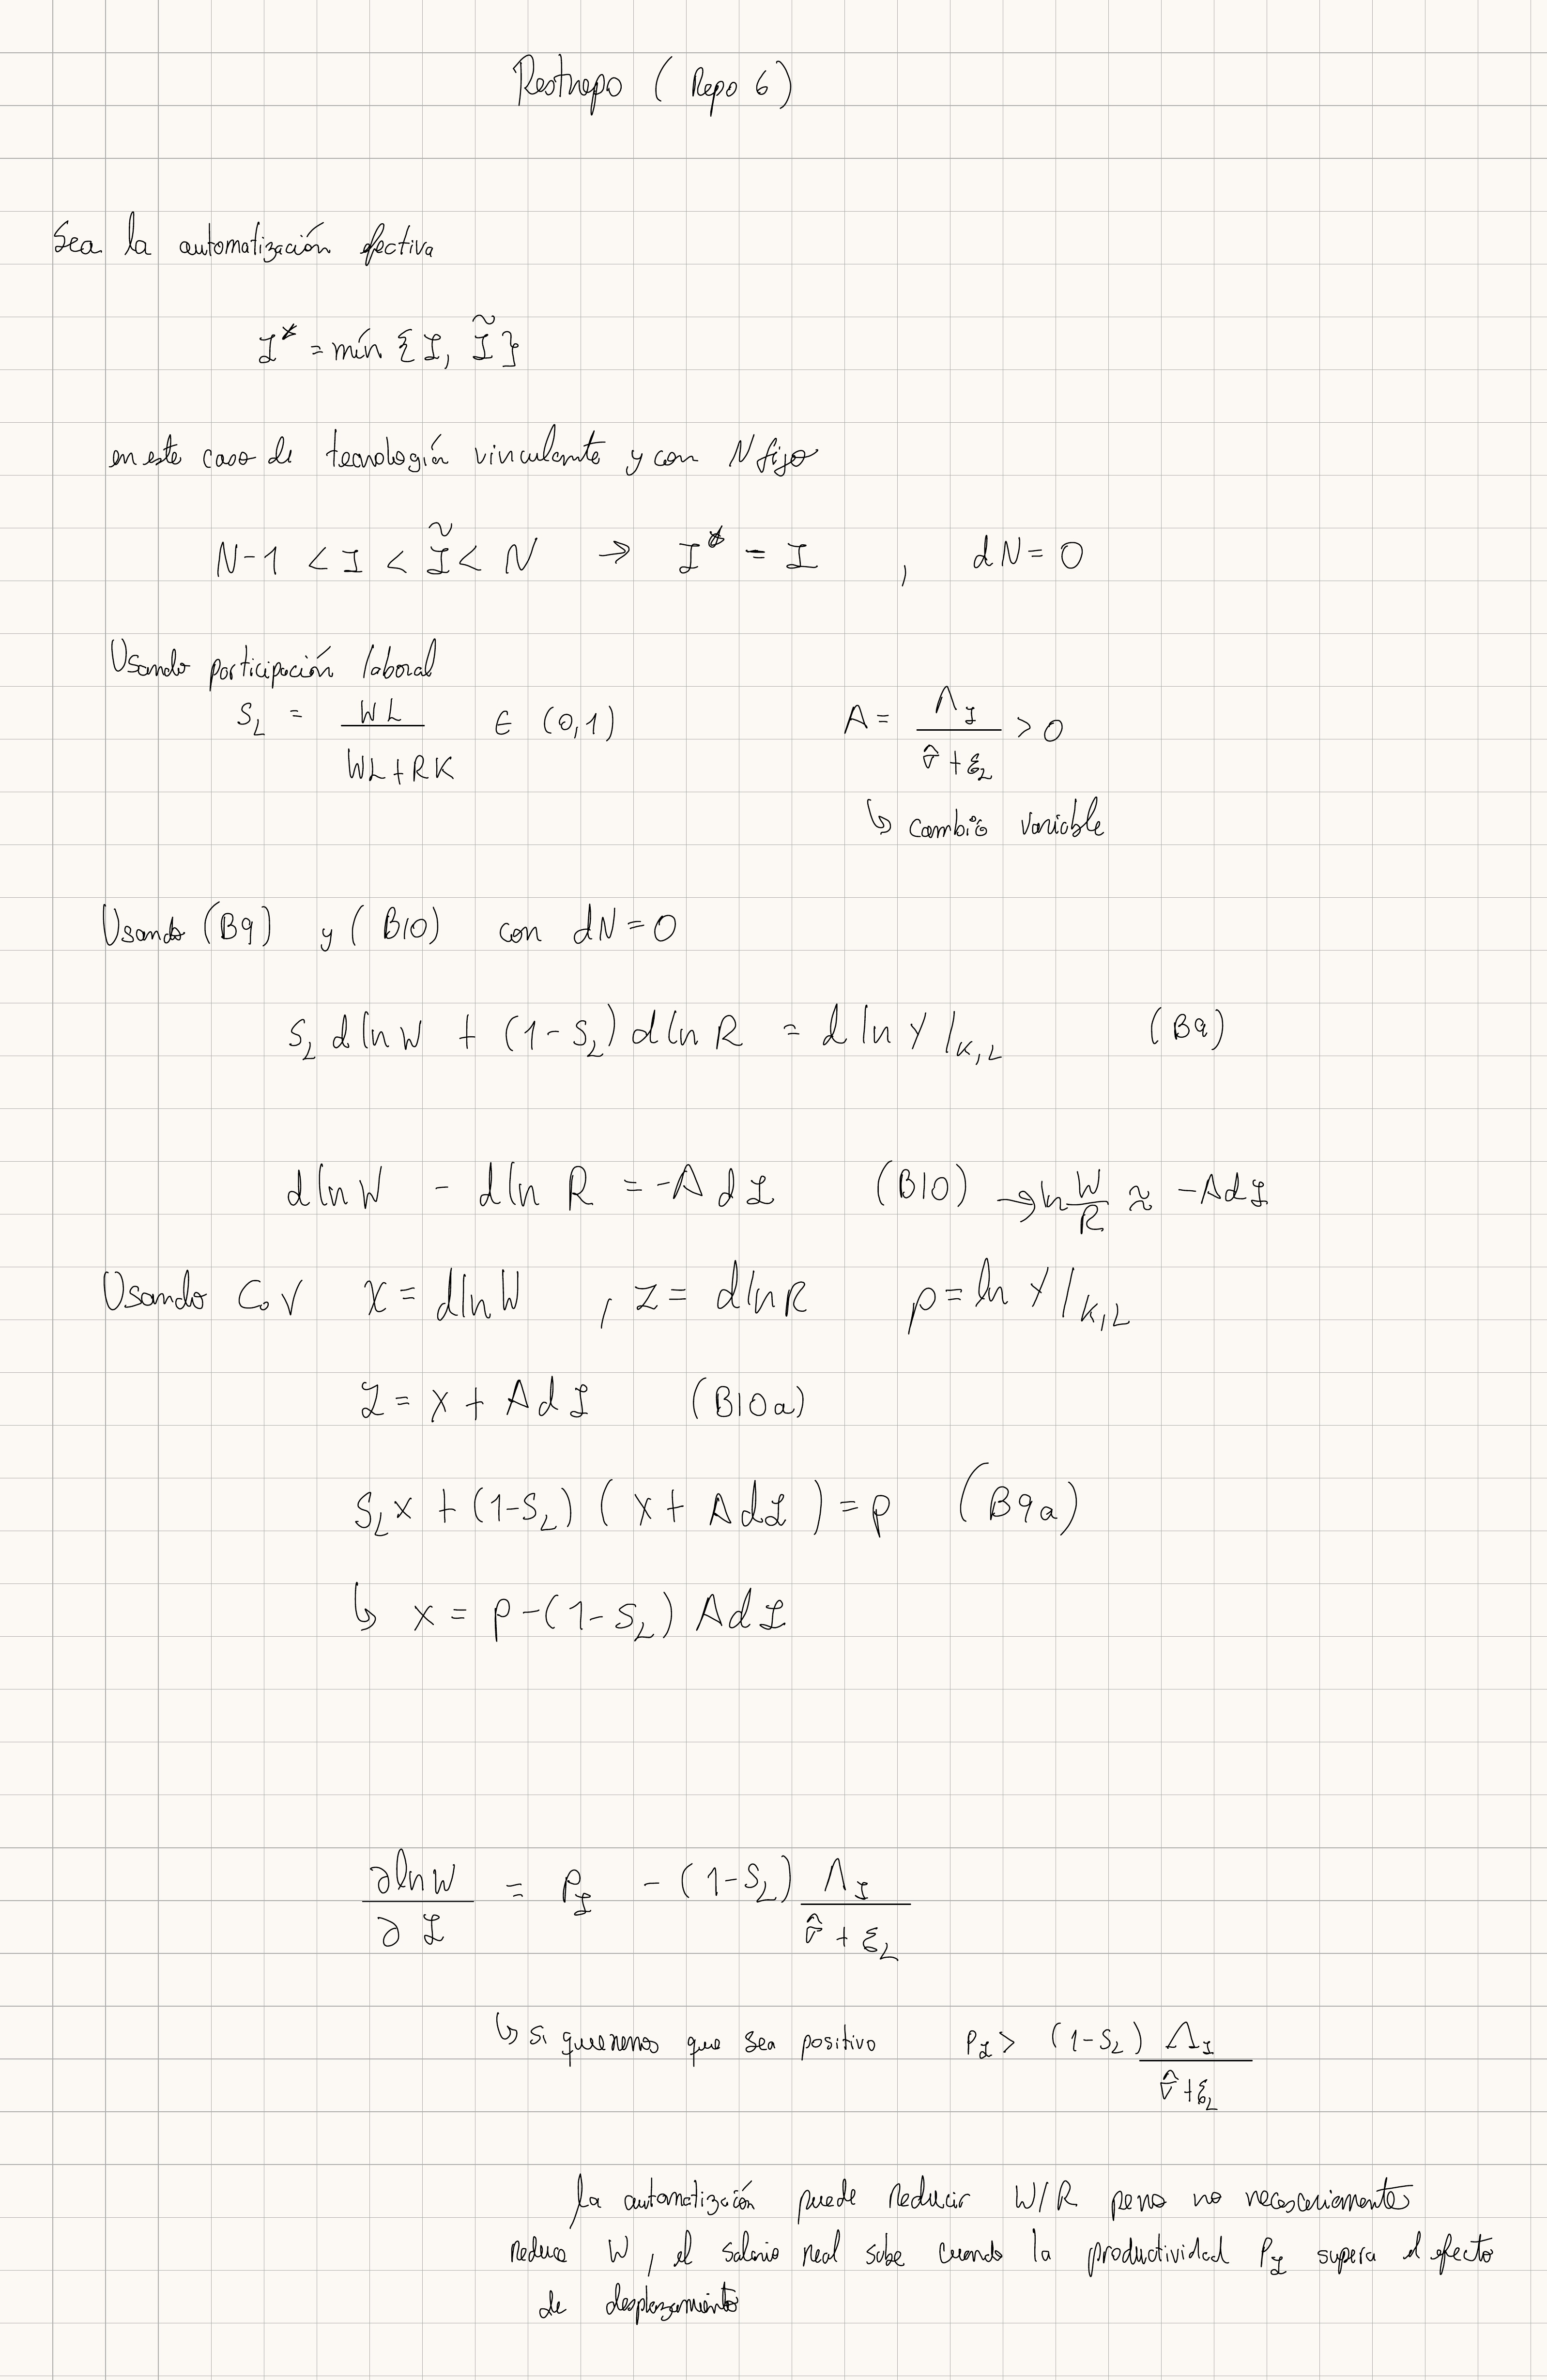
\includegraphics[height=.62\textheight]{hand/derivation.jpg}}{
\begin{center}\fbox{\parbox{.75\textwidth}{\centering Real photograph of the student's handwritten derivation pending. See \texttt{hand/README.md}.}}\end{center}}
\vspace{.3em}
\centering\small
$d\ln W/dI=P_I-D_I$, so a wage increase requires $P_I>D_I$.
\end{frame}

\IfFileExists{lean-slides.tex}{\begin{frame}{Lean 1/5: what entered the checker}
\begin{block}{Pinned source}
NBER Working Paper 22252, June 2017, 87 PDF pages. SHA-256 starts \texttt{441d0120}.
\end{block}
\begin{itemize}
\item AppliedModelingLib generated the complete \texttt{AR18RaceManMachine} paper folder.
\item The Lean target is Appendix B's algebra from (B9) and (B10) to the wage formula.
\item The code treats the differential values as real variables and takes (B9), (B10) as explicit hypotheses.
\end{itemize}
\vspace{.5em}
This is a checked \alert{support lemma}, not a proof that the economy satisfies those equations.
\end{frame}

\begin{frame}[fragile]{Lean 2/5: equation $\rightarrow$ statement $\rightarrow$ proof}
\vspace{-.5em}
\footnotesize
\[\underbrace{s_L d\ln W+(1-s_L)d\ln R=p}_{\text{(B9)}},\qquad
  \underbrace{d\ln W-d\ln R=q}_{\text{(B10)}}
  \quad\Longrightarrow\quad d\ln W=p+(1-s_L)q.\]
\vspace{-.5em}
\begin{lstlisting}
theorem wage_identity_from_B9_B10
    (s dW dR productivity relativePrice : Real)
    (hB9 : s*dW + (1-s)*dR = productivity)
    (hB10 : dW-dR = relativePrice) :
    dW = productivity + (1-s)*relativePrice := by
  linear_combination hB9 + (1-s)*hB10
\end{lstlisting}
\vspace{-.5em}
\footnotesize $s$ encodes labor's net-output share; $dW,dR$ encode the two log changes; $p$ is productivity; $q$ is the relative-price change. The slide spells Lean's $\mathbb R$ notation as \texttt{Real}. Lean verifies the algebra \emph{given} both premises.
\end{frame}

\begin{frame}{Lean 3/5: why the proof line works}
Write (B9) and (B10) as zero-valued residuals:
\begin{align*}
  A &= s\,dW+(1-s)\,dR-p,\\
  B &= dW-dR-q.
\end{align*}
The Lean proof uses $A+(1-s)B=0$. The $dR$ terms cancel and $s\,dW+(1-s)dW=dW$, leaving
\[dW-p-(1-s)q=0.\]
\vspace{.4em}
\texttt{linear\_combination} checks that weighted sum symbolically; it does not infer (B9) or (B10) from the task model.
\end{frame}

\begin{frame}[fragile]{Lean 4/5: the exact wage condition}
Set $q=-\Lambda_I/(\widehat\sigma+\varepsilon_L)$ for the binding-frontier case. The checked specialization gives
\[d\ln W=P_I-\frac{(1-s_L)\Lambda_I}{\widehat\sigma+\varepsilon_L}.\]
\small\textit{Excerpt below: binders and repeated arguments omitted for legibility.}
\begin{lstlisting}
theorem automation_wage_rises_iff ... :
    0 < dW <-> (1-s)*lambdaI/denominator
                 < productivity := by
  rw [automation_wage_change ...]
  constructor <;> intro h <;> linarith
\end{lstlisting}
\vspace{.4em}
\small The proposition is conditional on the encoded (B9) and (B10) identities. Its variables range over $\mathbb R$; positivity of $\widehat\sigma+\varepsilon_L$ is needed to derive (B10)'s sign from the economic primitives, not for this algebraic equivalence.
\end{frame}

\begin{frame}{Lean 5/5: results and open boundary}
\begin{block}{Machine results}
\texttt{lake build +AR18RaceManMachine}: passed.\\
\texttt{paper\_contribution.py check AR18RaceManMachine --fast}: passed.\\
Three support theorems use only \texttt{propext}, \texttt{Classical.choice}, and \texttt{Quot.sound}.
\end{block}
\vspace{.4em}
\begin{alertblock}{What remains open}
The full continuum equilibrium, its threshold comparative statics, and the derivation of (B9) and (B10) from the paper's model. No named result is claimed as fully proved. Source-to-Lean review and final closeout were not run.
\end{alertblock}
\end{frame}
}{%
\begin{frame}{Lean run: source to statement}
\begin{block}{Pending run}
The own-run formalization is in progress. This slide will show an actual source claim, exact Lean statement, and proof fragment after the check; no placeholder theorem is presented as verified.
\end{block}
\end{frame}
}

\begin{frame}{What the checks can and cannot conclude}
\begin{itemize}
\item The computational script verifies arithmetic on the stated wage identity.
\item Lean's compiler can verify a formal theorem only under its encoded assumptions and domain.
\item Matching the NBER claim requires a separate source-to-Lean comparison.
\item The full continuum equilibrium and all its comparative statics should be counted only if formally represented and proved.
\end{itemize}
\end{frame}

\begin{frame}{Conclusion}
\begin{block}{Economic result}
Automation reallocates tasks away from labor. With a binding frontier, labor share falls, while wages depend on the balance between productivity and displacement. New tasks reinstate labor.
\end{block}
\vspace{.5em}
\begin{block}{Methodological result}
The threshold, regime conditions, and sign inequality must all be explicit in any Lean translation or oral explanation.
\end{block}
\end{frame}

\begin{frame}{Sources}
\small
Acemoglu, D., and P. Restrepo (2018). ``The Race between Man and Machine: Implications of Technology for Growth, Factor Shares, and Employment.'' \emph{AER} 108(6), 1488--1542.\\[.6em]
Formalization source: NBER Working Paper 22252, revised June 2017, 87 pages. In particular Section 2, Propositions 1--3 and Appendix B.\\[.6em]
Course requirement: \url{https://github.com/alexanderquispe/AI-Econ-Modeling/issues/5}
\end{frame}

\end{document}
